\chapter{Model-Learning Framework}
\label{ch:methodology}

Our interest in this thesis lies in the development of probabilistic models for systems whose dynamics are stochastic.
The objective is to use a dataset of execution traces of a system to attain an accurate system representation, which can be used to obtain plans for optimal automated control of a system involving uncertainty.
In this chapter we describe our proposed framework that applies learning algorithms to obtain probabilistic models in the form of \acrshortpl{acr:mdp} and optimizes for a performance-maximizing model by sampling multiple hyper-parameter settings for these learning algorithms.

First off, in \autoref{sec:problem-statement} we define the problem at hand that the proposed framework aims to deal with.
Then, in \autoref{sec:application-mobile-robot}, the application of mobile robot navigation is introduced, which is one of the possible applications of the framework and is used as a running example in this chapter.
This application is also used for evaluating the proposed framework through the experiments that were carried out and are documented in \autoref{ch:experimental-results}.
Next, \autoref{sec:dataset-prerequisites} describes the prerequisites for the dataset serving as the input of the proposed model-learning framework.
Subsequently, in \autoref{sec:model-learning-routine}, a detailed description of the learning and optimization routine is provided which forms our \textit{base framework} for learning optimal \acrshortpl{acr:mdp}.
Finally, in \autoref{sec:multi-phase-framework}, we define our extension of this base framework in the form of a \textit{multi-phase framework} consisting of three phases whose aim is to further improve on the effectiveness of the framework.
%In \autoref{sec:model-learning-routine} a detailed explanation is provided of the learning and optimization routine which forms the basis of our framework.
%Then in \autoref{sec:cost-effective-optimization} the framework is extended such that it consists of three cost-incremental phases.
%Finally, in \autoref{sec:application-mobile-robot} a possible application (i.e., mobile robot navigation) of the framework is discussed, which is also used for evaluating the approach through the experiments that have been carried out and which are described in \autoref{ch:experimental-results}.
%vTODO Avoid 'cost-incremental'

\section{Problem Statement}
\label{sec:problem-statement}

%vTODO State clearly again our problem, what we are going to do and why we want to do it (but in little more detail where necessary than in the introduction).
%vTODO Formalize the problem
%vTODO Say something about related work moving to reinforcement learning -> issues with this (perhaps: RL takes long and involves 'dangers' as it is done in the real-world; BRL intractable)
%TODO Go over this later on
As mentioned in \autoref{ch:introduction}, the problem this thesis is concerned with is the development of probabilistic models in the form of \acrshortpl{acr:mdp} to be used for obtaining plans for automated control of systems that involve uncertainty.
The development of such probabilistic models tend to be a difficult and time-costly process for a human designer.
Therefore, an appealing idea is to automate the model development process by applying learning algorithms on a dataset of execution traces of the system in need of automated control.
However, to achieve effective planning in a real-world environment, the models that are learned should accurately reflect the dynamics of the system, such that derived plans account for the uncertainty that is present in the execution of actions, observations and exogenous events.
Although algorithms for learning \acrshortpl{acr:mdp} from a dataset do already exist, the state of the art lacks a method of setting the hyper-parameters $\theta$ of these algorithms such that a model is retrieved that best reflects the underlying system and maximizes the performance in its execution of derived plans.
Besides, although \acrfull{acr:rl} allows us to bypass the development of a model, it often turns out to be quite slow for finding optimal policies in complex environments.
%Therefore, when one is able get a hold on a dataset describing the dynamics of the system under consideration, it may be better to take advantage of this by developing a probabilistic model.% and possibly further adjust it based on new experience as seen in \autoref{sec:active-learning}.
More formally, summarizing the above, the problem can be formulated as follows:

\begin{problem}
	Given a set $E$ of execution traces describing the dynamics of a system that involves uncertainty, an \acrshort{acr:mdp} $\mathcal{M}$ needs to be developed, utilizing learning algorithms parameterized by a set of hyper-parameters $\theta$ configured in such way to maximize the performance yielded by following the policies computed from this model $\mathcal{M}$ in a real-world setting.
\end{problem}

All in all, the problem we deal with is that of automating the task of learning a performance-maximizing \acrshort{acr:mdp} that generalizes well over multiple tasks for a system involving uncertainty.
This involves the need for a proper performance measure to express the value of a learned \acrshort{acr:mdp} and allow for a fair comparison of different \acrshortpl{acr:mdp}.
That is, depending on the parameter-settings of the learning algorithm used, an \acrshort{acr:mdp} may yield low performance in its execution for two major reasons.
First of all, the learned model may be too complicated for the amount of available data, which leads to model over-fitting.
On the other hand, one could acquire a model that is too simple to explain the available data and so does not accurately reflect the underlying system in that situation.
Therefore, the parameters of the learning algorithm should be properly adjusted in order to obtain accurate probabilistic models.
Finally and most importantly, a solution to this problem should take into account the costs of learning and evaluating these system models.

\section{Application to Mobile Robot Navigation}
\label{sec:application-mobile-robot}
% Use the mobile robot navigation domain as a **running example** application rather than putting it in the last section of the chapter

\begin{figure}[t]
	\centering
	
	\captionsetup{font=small}
	\captionsetup[subfigure]{font=footnotesize}
	\captionsetup[subfigure]{justification=centering}
	\begin{subfigure}{.5\textwidth}
		\centering
		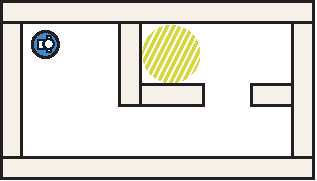
\includegraphics[width=.8\linewidth]{dummy-map-2-1}
		\caption{Dummy environment with a mobile robot and goal area.}
		\label{fig:dummy-map-1}
	\end{subfigure}\hfill
	\begin{subfigure}{.5\textwidth}
		\centering
		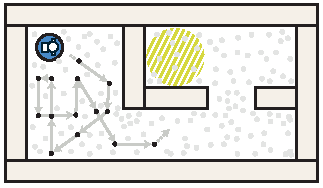
\includegraphics[width=.8\linewidth]{dummy-map-2-2v2}
		\caption{Data-points of execution traces from exploration depicted.}
		\label{fig:dummy-map-2}
	\end{subfigure}
	
	\bigskip
	
	\begin{subfigure}{.5\textwidth}
		\centering
		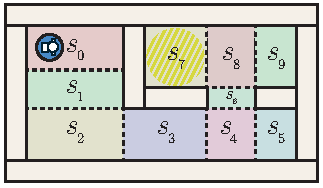
\includegraphics[width=.8\linewidth]{dummy-map-2-3}
		\caption{State-space of a learned \acrshort{acr:mdp} depicted.}
		\label{fig:dummy-map-3}
	\end{subfigure}\hfill
	\begin{subfigure}{.5\textwidth}
		\centering
		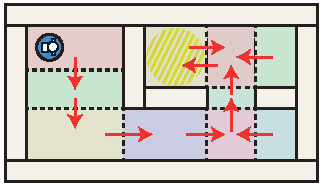
\includegraphics[width=.8\linewidth]{dummy-map-2-4}
		\caption{Corresponding optimal policy for the \acrshort{acr:mdp}.}
		\label{fig:dummy-map-4}
	\end{subfigure}
	\caption{Planning for the navigation of a mobile robot by learning \acrshortpl{acr:mdp} from data about the environment.}
\end{figure}

%\begin{itemize}
%	\item Description
%	\item Motivation of this application
%	\item Generalization to other applications
%	\item Details on how we apply the framework to this application
%\end{itemize}

%vTODO Throughout this chapter
%vTODO Use formal notation to clarify
In this chapter a model learning framework is proposed that could be employed for various planning problems involving uncertainty.
To illustrate the type of problems this framework is aimed at and what comprises a probabilistic model for such problems, we use its application to path planning in mobile robot navigation as a running example throughout this chapter.
%An example application for which the model learning framework described in this chapter could be used is that of mobile robot navigation.
The problem statement for this application is as follows: a mobile robot needs to be autonomously controlled by an agent in such way to navigate from one location to another in some world, say, an office environment, as fast as possible.
This problem domain is particularly suited as the robots tend to operate under significant uncertainty in their actions (e.g., slipping) and observations (e.g., sensor noise).
Although there are other potential applications as described in \autoref{ch:introduction}, this particular application can be used to illustrate the procedure of learning \acrshortpl{acr:mdp} from data and obtaining plans accordingly quite well.

For example, let us consider the scenario in which the robot needs to operate in an environment as depicted in \autoref{fig:dummy-map-1}.
For now let us assume, the action space $A$ is defined as a finite set of movements in the cardinal and inter-cardinal directions, such that: 
\begin{align*}
%	A = \{&\texttt{SOUTH}, \texttt{SOUTH-EAST}, \texttt{EAST}, \texttt{NORTH-EAST}, \\
%	&\texttt{NORTH}, \texttt{NORTH-WEST}, \texttt{WEST}, \texttt{SOUTH-WEST}\}
	A = \{&\texttt{S}, \texttt{SE}, \texttt{E}, \texttt{NE},
		  \texttt{N}, \texttt{NW}, \texttt{W}, \texttt{SW}  \}
\end{align*}\newpage
Before our model learning framework is applied to learn \acrshortpl{acr:mdp} for the system, the data about the environment could have been obtained in the form of execution traces that consist of logs of the robot's pose and the (next) action it is about to take.
This could then give a set of data-points, as depicted in \autoref{fig:dummy-map-2}, which can be used to learn the states and transition probabilities of an \acrshort{acr:mdp}.
Quantizing this dataset of observed robot poses into $10$ symbols (e.g., using $k$-means clustering), might give us the state-space $\mathcal{S} = \{s_0, \ldots s_9\}$ depicted in \autoref{fig:dummy-map-3}.
%, such that:
%$$
%\mathcal{S} = \{s_0, \ldots s_9\}
%$$
%A potential state-space of an \acrshort{acr:mdp} that might be learned from this dataset is shown in \autoref{fig:dummy-map-3}.
Accordingly, based on such a quantization into a state-space $\mathcal{S}$, one can learn a transition function $\delta: \mathcal{S} \times A \times \mathcal{S} \mapsto [0, 1]$ for an \acrshort{acr:mdp} applying the maximum-likelihood estimation as described in \autoref{sec:learning-markov-models}.
Then, say that for instance, we define a task for the robot as moving from an initial position in state $s_0 \in \mathcal{S}$ to a goal area corresponding to the state $s_7 \in \mathcal{S}$ as depicted.
This would make us define a reward function $R: \mathcal{S} \times A \times \mathcal{S} \mapsto \mathbb{R}$ for our \acrshort{acr:mdp} such that only a reward can be obtained from the `goal' state $s_7$, i.e.:
\[
R(s, a, s') = 
\begin{cases}
\hspace{4pt} 	1 & \text{if } s' = s_7 \land s \neq s'\\
\hspace{4pt} 	0 & \text{otherwise}
\end{cases}
\]

Putting the earlier defined components together, an \acrshort{acr:mdp} $\mathcal{M}$ for this particular task is $\mathcal{M} = (\mathcal{S}, s_0, A, \theta, R)$.
Accordingly, an optimal policy $\pi^\ast$, defining the most appropriate action from any state, is quite straightforward for this simple \acrshort{acr:mdp} and is depicted in \autoref{fig:dummy-map-4}.
%Then, assigning a reward to a state that covers the goal area should give us a policy that leads the robot from any initial state to the goal state as depicted in \autoref{fig:dummy-map-4}.

In this application the value of a learned \acrshort{acr:mdp} needs to depend on how fast the robot would reach its goal location for the various tasks it is expected to perform.
It should be noted that a proper assessment of model value should be made based on the performance in simulations and the real world as there may exist discrepancies between states in the model and the actual state of the system in its execution.
In the following sections we discuss how the proposed framework takes these aspects into account so that on convergence an \acrshort{acr:mdp} is obtained that reflects the real world and generalizes over multiple tasks quite well. %TODO Update last sentence with new contents of chapter

%In this application the performance of a learned \acrshort{acr:mdp} can be assessed as described in \autoref{sec:performance-measure} through the computed value function and performing simulations for the various tasks the robot should be able to execute.
%Comparing the performance that was assessed for multiple \acrshortpl{acr:mdp} through the framework on convergence leads to an \acrshort{acr:mdp} that reflects the real world and generalizes over multiple tasks quite well.

\section{Dataset Prerequisites}
\label{sec:dataset-prerequisites}
% vTODO Explain how we would like to see the exploration/data acquisition to be performed. Dataset should appropriately ('of sufficient quality') reflect the dynamics of the system so that an accurate representation in the form of an MDP can be learned from it.

% Type of content
Prior to describing the proposed framework for the problem as specified in \autoref{sec:problem-statement}, we are obliged to specify the expected format of the datasets to learn \acrshortpl{acr:mdp} from.
A self-evident approach is making use of a dataset generated from execution traces, in which the system under consideration logged a set of readings/observations describing the system state accompanied by the actions selected in between at a fixed time interval.
One should note that this means that the action space $A$ and time step $t$, that will be used for any \acrshort{acr:mdp} for the system, should already have been established at this point.
When adding the auxiliary condition of needing to learn fully-observable \acrshortpl{acr:mdp}, the need arises for the observations in these execution traces to be usable for distinguishing between the different system states.

For our running example of mobile robot navigation such a dataset may be obtained by executing the robot in its real-world environment following a random action policy.
That is, one could choose to let the robot record its location and orientation in terms of its sensor readings which are logged at a fixed time interval.
In the exploration, the robot would then start from some position in the environment, choose an action (e.g., driving forward in some direction) at random and execute it according to the fixed time step.
What would then be logged are the robot's sensor readings and selected action at each stage.
Recording the action at each stage is appropriate as it allows us to observe the effect of the actions and identify actions that do not affect the robot's state (e.g., being unable to move because of a wall or other obstacle close to the robot).

% Size of content
Further, one should ensure that the dataset obtained from the exploration at least holds observation-action pairs for the area of the observation/state space of interest for the tasks the system is expected to perform.
For our running example, this would be covering most of the reachable parts of the environment and trying out actions in each area multiple times.
Clearly, one could decide to exclude or limit exploration for those areas that are deemed not of interests for the tasks the system is expected to perform.
All in all, the learning algorithm requires one to fix an action space $A$ and time step $t$ and gather a dataset consisting of a sufficient number of observation-action pairs to describe the dynamics of the system under consideration.

\newpage

\section{Base Framework}
\label{sec:model-learning-routine}
%vTODO Formalize the methodology

\begin{algorithm}[t!]
	\caption{\acrshort{acr:mdp}-Optimization Base Framework}
	\label{alg:base-framework}
	\begin{algorithmic}[1]
		\Require{Set of execution traces $E$, Parameter space $\Theta$, Set of tasks $T$, Action space $A$, Time-step $t$, Discount factor $\gamma \in [0, 1]$, Weight factor $\beta \in [0, 1]$, Acquisition function $a: \Theta \mapsto \mathbb{R}$}%Training set $\mathcal{O} = \{O_1, \ldots, O_k\}$, Clustering algorithm, hyper-parameter(s) $\theta$, actions $A$}
		\Ensure{\acrshort{acr:mdp} $\mathcal{M}_\mathsf{max}$, Evidence set $\mathcal{D}$}%\acrshort{acr:mdp} $\mathcal{M} = (\mathcal{S}, s_0, A, \delta, R)$} \Comment{$s_0$ and $R$ are here irrelevant}
		\State $\mathcal{M}_\mathsf{max} \gets \texttt{NULL}$
		\State $V_{\mathcal{M}_\mathsf{max}} \gets 0$
		\State $\mathcal{D} \gets \emptyset$ \Comment{The evidence set storing samples and observations}
		\State $\mathit{gp} \gets GP(0, K)$ \Comment{Zero-mean \acrshort{acr:gp} with covariance $K$}
		\State Sample $\theta \in \Theta$ at random
		\Repeat
		\State $\mathcal{M}, V_\mathcal{M} \gets \textproc{LearningStep}(\theta)$
		\If{$V_\mathcal{M} > V_{\mathcal{M}_\mathsf{max}}$}
		\State $V_{\mathcal{M}_\mathsf{max}} \gets V_\mathcal{M}$
		\State $\mathcal{M}_\mathsf{max} \gets \mathcal{M}$
		\EndIf
		\State $\theta \gets \textproc{OptimizationStep}(\theta, V_\mathcal{M}, \mathcal{D}, \mathit{gp})$
		\Until{convergence}
		\State\Return $\mathcal{M}_\mathsf{max}, \mathcal{D}$
		\Statex
		\Function{LearningStep}{$\theta$}	\label{alg:line:learn}
			\State $\mathcal{S} \gets \textproc{Quantization}(E, \theta)$
			\State $\delta \gets \textproc{MaxLikelihood}(E, \mathcal{S}, A, \theta)$
			\State $V_\mathit{DTP} \gets 0$
			\State $V_\mathit{SIM} \gets 0$
			\ForAll{$(\mathit{start}, \mathit{goal}) \in T$}
			\State $\{s_0, s_g\} \gets \textproc{ToStates}(\{\mathit{start}, \mathit{goal}\})$
			\State $R \gets \textproc{ToRewardFunction}(s_g)$
			\State $\mathcal{M} \gets (\mathcal{S}, s_0, A, \delta, R)$
			\State $V, \pi \gets \textproc{DTPPlanning}(\mathcal{M})$	\Comment{Solve for a policy $\pi$ using a \acrshort{acr:dtp} algorithm, such as \acrshort{acr:vi}}
			\State $V_\mathit{DTP} \gets V_\mathit{DTP} + V[s_0]$
			\If{$\beta < 1$}
				\State $\mathsf{task\_status}, \mathit{steps} \gets \textproc{RunSim}(\mathcal{M}, \pi)$
				\If{$\mathsf{task\_status} = \texttt{success}$}
					\State $V_\mathit{SIM} \gets V_\mathit{SIM} + \gamma^\mathit{steps} \cdot R[s_g]$
				\EndIf
			\EndIf
			\EndFor
			%\State $V_\mathit{DTP} \gets \frac{V_\mathit{DTP}}{|T|}$
			%\State $V_\mathit{SIM} \gets \frac{V_\mathit{SIM}}{|T|}$
			%\State $V_\mathcal{M} \gets \beta \cdot V_\mathit{DTP} + (1 - \beta) \cdot V_\mathit{SIM}$
			\State $V_\mathcal{M} \gets \beta \cdot \frac{V_\mathit{DTP}}{|T|} + (1 - \beta) \cdot \frac{V_\mathit{SIM}}{|T|}$
			
			\State\Return $\mathcal{M}, V_\mathcal{M}$
		\EndFunction
		\Statex
		\Function{OptimizationStep}{$\theta, V_{\mathcal{M}}, \mathcal{D}, \mathit{gp}$}
			\State $\mathcal{D} \gets \mathcal{D} \cup \{(\theta, V_\mathcal{M})\}$
			\State $\mathit{gp}.\textproc{fit}(\mathcal{D})$	\Comment{Fit a \acrshort{acr:gp} given $\mathcal{D}$, maximizing the log-marginal-likelihood}
			\State\Return $\argmax_{x \in \mathcal{\Theta}} a(x \vert \mathcal{D}, \mathit{gp})$	\Comment{Suggest a sample $\theta$ to evaluate next}
		\EndFunction
	\end{algorithmic}
\end{algorithm}

\begin{figure}[t]
	\centering
	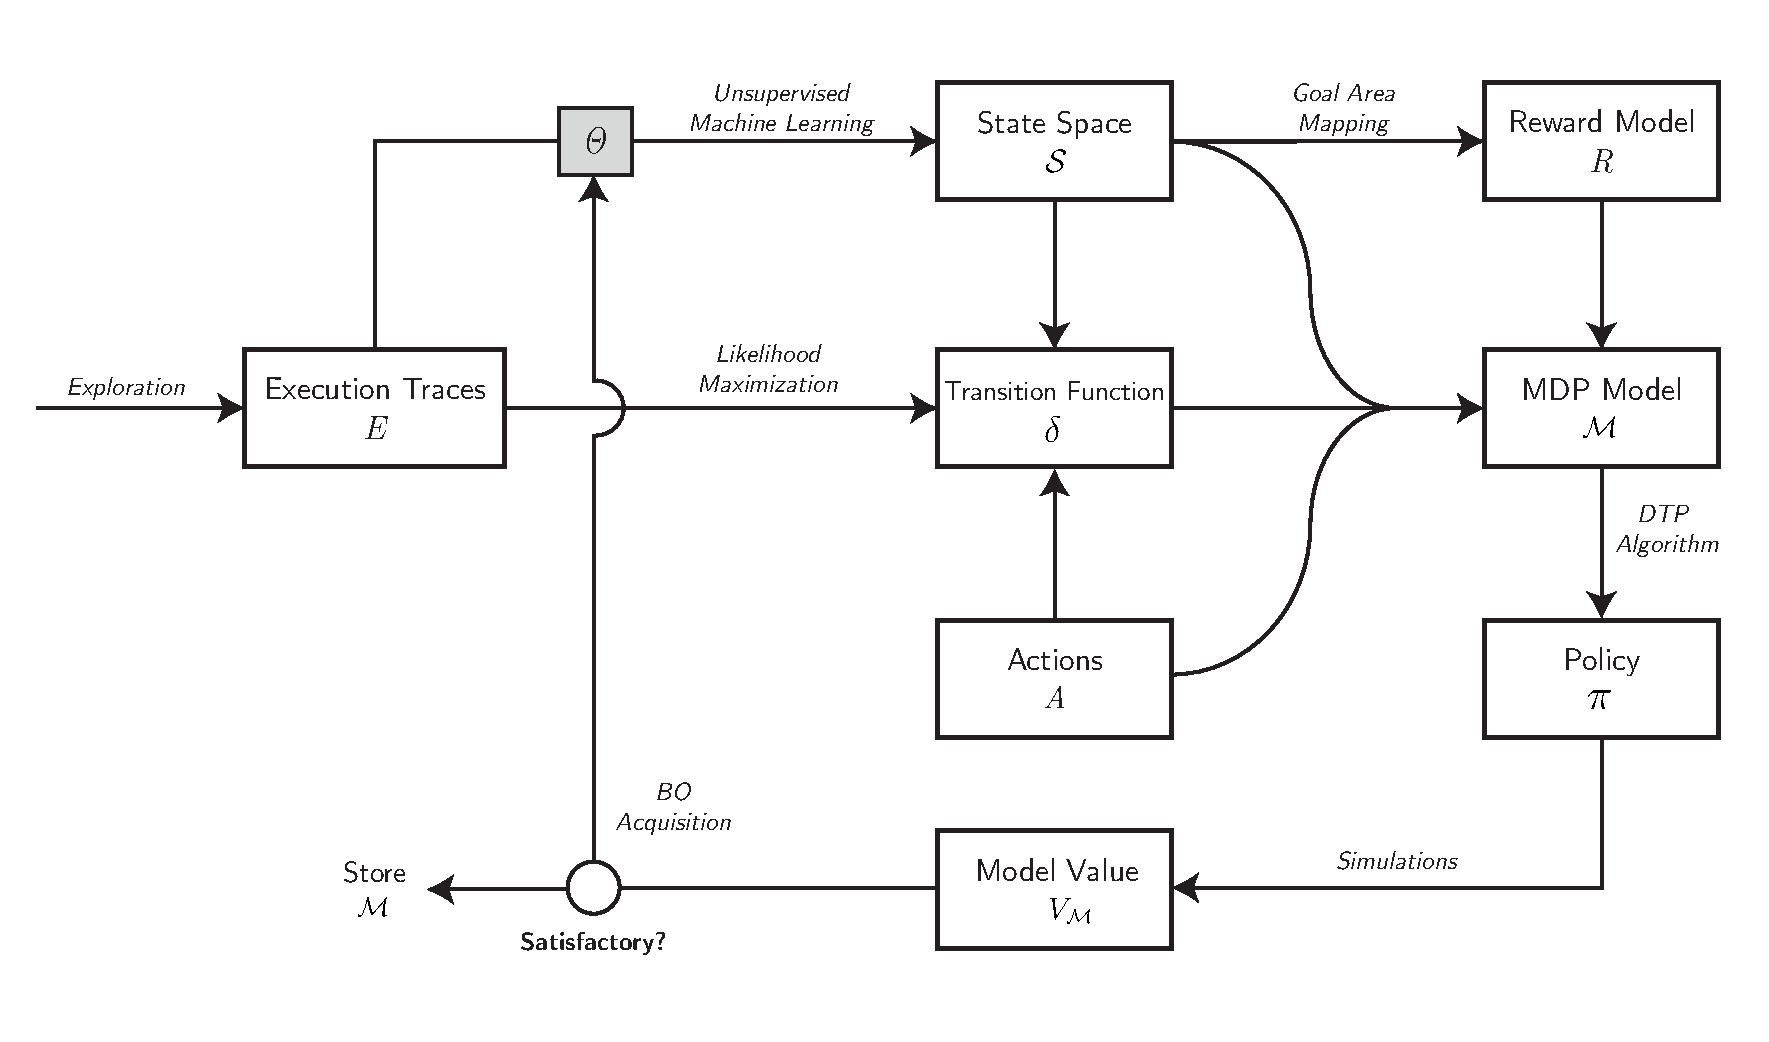
\includegraphics[width=\textwidth]{learning-cycle-complete-v23}
	\caption{Schematic diagram of the model learning and optimization routine.}
	\label{fig:learning-routine-complete}
\end{figure}

The learning and optimization routine described in this section forms the \textit{base framework} for the problem dealt with.
This routine, schematically depicted in \autoref{fig:learning-routine-complete}, aims to properly adjust the hyper-parameters $\theta$ of the employed model learning algorithm by posing it as an optimization task.
The objective is then to obtain an \acrshort{acr:mdp} that maximizes the performance of executing the plans that are derived from it.
In the remainder of this section we explain the working of this routine of which the corresponding pseudo-code is presented in \autoref{alg:base-framework}.

%The learning and optimization routine described in this section, depicted in \autoref{fig:learning-routine-complete}, aims to achieve this by posing the adjustment of these parameters as an optimization task, with the objective of obtaining an \acrshort{acr:mdp} model that maximizes the performance of executing the plans that are derived from it.

\subsection{Learning Step}
\label{sec:learning-step}
%vTODO Explain the components that we learn/derive (state space and transition function and accordingly reward functions) and which components are fixed (actions)

The routine can be viewed as consisting of two subsequent steps which are repeated until an \acrshort{acr:mdp} model that yields satisfactory performance is obtained.
The first of these two main steps will be referred to as the \textit{learning step}, in which an \acrshort{acr:mdp} model is learned and its value is assessed.

This learning step starts off with a data-set of execution traces $E$ obtained beforehand as described in \autoref{sec:dataset-prerequisites}.
As we can see in \autoref{alg:base-framework}, \autoref{alg:line:learn}, the step is parameterized by $\theta$, which represents the parameter-setting to be used for the employed model learning algorithm.
Given a parameter-setting $\theta$, a state-space $\mathcal{S}$ is acquired by quantizing the execution traces $E$ using an unsupervised machine learning algorithm.
Subsequently, a transition function $\delta$ is acquired by applying a known model-learning algorithm (such as one of those described in \autoref{sec:learning-probabilistic-models}) given the data-set $E$, state-space $\mathcal{S}$ and possible actions $A$.
The tasks to perform are each accordingly mapped to a reward function $R$ over the acquired state-space $\mathcal{S}$ (or alternatively over state-action pairs or state-action-state triplets).
The state-space $\mathcal{S}$, transition function $\delta$, action set $A$, reward function $R$ and a configurable initial state $s_0$ are then combined into an \acrshort{acr:mdp} $\mathcal{M} = (\mathcal{S}, s_0, A, \delta, R)$.

To assess the performance yielded by $\mathcal{M}$, the \acrshort{acr:mdp} is solved by applying known \acrshort{acr:dtp} algorithms like \acrshort{acr:vi} or \acrshort{acr:pi} to obtain policies for a set of tasks the system is expected to perform.
The value of the model $V_{\mathcal{M}}$ is then determined by checking how well the system is expected to perform by execution according to the derived policies (e.g., based on simulations and/or the value function obtained by a \acrshort{acr:dtp} algorithm).
The sections below describes each of the components of this algorithm in more detail and most importantly defines the performance measure that is used for assessing the value of learned \acrshortpl{acr:mdp}.
%\autoref{sec:performance-measure} describes in detail how the performance yielded by the learned \acrshortpl{acr:mdp} is assessed and how a fair comparison of different \acrshortpl{acr:mdp} may be achieved for this routine.

%~TODO Finish and refer to algorithm environment
%vTODO Explain where each component of the MDP comes from
%vTODO Devote a paragraph clearly on how the reward function is defined; multiply the reward with the discrepancy factor rather than the value 

\subsubsection{Action-Space and Time Step}
The action space $A$ of the \acrshort{acr:mdp} to be learned is one of the input parameters for the framework and should match the actions used in obtaining the set $E$ of execution traces.
Similarly, the time step $t$ is an input parameter as well, which specifies the time in between stages in which the agent selects an action, again matching the time step used in obtaining the set $E$ of execution traces.
In our running example, one possibility is to define the action space as the set of movements in the cardinal and inter-cardinal directions as seen earlier in \autoref{sec:application-mobile-robot}.
The time step $t$ for the mobile robot would then correspond to the period of time it moves in one of these directions after it has selected an action $a \in A$.

\subsubsection{State-Space}
From the provided set of execution traces $E$, a state-space $\mathcal{S}$ is learned based on the current hyper-parameter setting $\theta$ in the learning step.
For instance, in our running example, a $k$-means clustering can be applied on for instance, coordinates in the execution traces $E$ describing the reachable locations of the robot, where $k$ is specified by the setting of $\theta$.

\subsubsection{Transition Function}
In the learning step the transition function $\delta$ is obtained by applying a known model-learning algorithm, for which here a likelihood maximization approach is selected for learning the transition probabilities of a fully observable \acrshort{acr:mdp}.
The transition function is defined for the provided action space $A$ and earlier acquired state-space $\mathcal{S}$ and approximated from the transitions in the set $E$ of execution traces.
%Depending on the application, one could choose to apply another algorithm

\subsubsection{Tasks and Reward Functions}

\begin{figure}[t!]
	\centering
	\begin{tikzpicture}[->,>=stealth',auto,node distance=2.5cm,every label/.style=draw,every initial by arrow/.style={dashed}]
	\tikzstyle{every state}=[fill=white,draw=black,text=black,scale=1]	% thick
	\node[state,initial,initial text={},label={50:\small$+0$}] (s1) {};
	\node[state,initial,initial text={},label={50:\small$+0$}] (s2) [below of=s1] {};
	\node[state,initial,initial text={},label={50:\small$+0$}] (s3) [right of=s1] {};
	\node[state,label={50:\small$+1$}] (goal) [below of=s3] {G};
	\node[state,label={50:\small$+0$}] (trap) [right of=goal] {\text{T}};
	\coordinate (con) at (0,2);
	\path
	(s1)
	edge node {$a_i$} (goal)
	(s2)
	edge node {$a_j$} (goal)
	(s3)
	edge node {$a_k$} (goal)
	(goal)
	edge node {$A$} (trap)
	(trap)
	edge [loop above] node {$A$} (trap)
	;
	%\draw [->, dashed, shorten >=0pt] (s3) to[right] node[auto] {} ++(1.3,0)
	;
	\end{tikzpicture}
	\caption{One-time reward in goal state G in an \acrshort{acr:mdp} realized by an absorbing state T.}
	\label{fig:goal-trap-state}
\end{figure}

The goal for the class of problems of interest is to obtain a well-generalizing model that performs well on multiple different tasks.
Therefore, an estimate of the value of a model is assessed over a set $T$ of tasks provided as input to the framework, where each task is presented as the combination of a starting and goal configuration.
%To achieve this, let us first define multiple starting configurations and multiple goals for the system.

The starting configurations are each mapped to corresponding states in the \acrshort{acr:mdp}, matching the quantization to state-space $\mathcal{S}$, so that one can define $\mathcal{S}_0 \subseteq \mathcal{S}$ as a set of initial states.
Similarly, the goals are each mapped to states, such that one can define $\mathcal{S}_G \subseteq \mathcal{S}$ as a set of goals.
One problem that emerges, however, is that there might not be a one-to-one correspondence between learned and true (goal) states, which leads to the possibility of small state spaces yielding high value while the goal states might not map well to the true goal states.
To take care of this, we introduce a discrepancy factor $\xi \in [0, 1]$, which corresponds to the fraction of entries from the set $E$ within the goal state that map to the true goal.

Let us then define $R_G$ as the set of reward functions $R_i$ for each $i \in \mathcal{S}_G$ in which a one-time reward (which is realized as depicted in \autoref{fig:goal-trap-state}) is received only in goal-state $i$.
Note that as such, an equivalent formulation can be given as a \textit{stochastic shortest path} problem \cite{GuillotS17} for the resulting \acrshortpl{acr:mdp}.
The reason the reward needs to be only obtainable once is to ensure that the expressions $V_\mathit{DTP}$ and $V_\mathit{SIM}$ are in the same range and can be used together as discussed in the next section.
%The reward function $R_i: \mathcal{S} \mapsto \mathbb{R}$ for some task with goal state $i \in \mathcal{S}_G$ is then defined as follows:
%\begin{equation}
%R_i(s) = 
%\begin{cases}
%\hspace{4pt} \xi & \text{if } s = i \\
%\hspace{4pt} 0 & \text{otherwise}
%\end{cases}
%\end{equation}
The reward function $R_i: \mathcal{S} \times A \times \mathcal{S} \mapsto \mathbb{R}$ for some task with goal state $i \in \mathcal{S}_G$ is then defined as follows:
\begin{equation}
R_i(s, a, s') = 
\begin{cases}
\hspace{4pt} \xi & \text{if } s' = i \\
\hspace{4pt} 0 & \text{otherwise}
\end{cases}
\end{equation}

Accordingly one can define $T_{\mathcal{M}} = \mathcal{S_0} \times R_G$ as the set of tasks, in the form of all pairs of initial states and reward functions, over which the performance is assessed.
The next section discusses how the value of a model $\mathcal{M}$ is assessed in the learning step over these tasks.

\newpage %

\subsubsection{Performance Measure}

Posing the learning of probabilistic models as an optimization task requires us to define a mapping of \acrshortpl{acr:mdp} to a performance measure that can fairly compare different models.
As discussed earlier, one can express the performance of an \acrshort{acr:mdp} in terms of how well the agent performs tasks following the policies that are derived from the model.
Therefore, one option is to make use of the value function $V$ obtained by a \acrshort{acr:dtp} algorithm, such as \acrshort{acr:vi} or \acrshort{acr:pi}.
Based on such a value function, an expression of how well the agent is expected to perform some task $t = (s_0, R) \in T_\mathcal{M}$ is:
\begin{equation}
\label{eq:vdtp}
V_{\mathit{DTP}, t=(s_0, R)} = V[s_0]
\end{equation}
where $s_0 \in \mathcal{S}$ is the initial state and $R$ the reward function of the \acrshort{acr:mdp} for the task.

However, although the \acrshort{acr:dtp} algorithm may yield high value for the task, it might be that the agent will not perform well following the policy in the real world.
To better assess the performance, one could execute simulations in which the agent follows the policy derived from the \acrshort{acr:mdp} model.
Although performing simulations is more cost-expensive, it yields a better approximation of how well the agent executes a task following a policy obtained from the model.
Accordingly, let us express the performance on some task in simulations as:
\begin{equation}
\label{eq:vsim}
V_{\mathit{SIM}, t=(s_0, R)} = \gamma^{k} \cdot R[i]
\end{equation}
where $s_0 \in \mathcal{S}$ is the initial state, $R$ the reward function, $\gamma$ the discount factor, $i \in \mathcal{S}$ the goal state and $k$ the number of steps taken to reach the goal.

Combining the expressions of \autoref{eq:vdtp} and \autoref{eq:vsim} yields the following expression of the performance on some task $t \in T_\mathcal{M}$:
\begin{equation}
\label{eq:vcom}
\beta \cdot V_{\mathit{DTP}, t=(s_0, R)} + (1 - \beta) \cdot V_{\mathit{SIM}, t=(s_0, R)}
\end{equation}
where $\beta \in [0, 1]$ is a parameter which specifies the relative weight of $V_{\mathit{DTP}, t}$ against that of $V_{\mathit{SIM}, t}$ and where $s_0$ and $R$ are the initial state and reward function for the task respectively.

\noindent Putting this all together, the performance of an \acrshort{acr:mdp} $\mathcal{M}$ can in this way be expressed as:
\begin{equation}
\label{eq:vm}
V_{\mathcal{M}} = \frac{\sum_{t \in T_\mathcal{M}} \beta \cdot V_{\mathit{DTP}, t} + (1 - \beta) \cdot V_{\mathit{SIM}, t}}{|T_\mathcal{M}|}
\end{equation}
where $T_\mathcal{M}$ is the set consisting of the pairs of initial states and reward functions of the tasks over which the performance is assessed.

%\begin{itemize}
%	\item Start off with data-set of execution traces obtained beforehand
%	\item A number of parameter-settings $\theta$ for the model-learning are initially sampled at random from a designer-specified domain $\Theta$ (i.e., the parameter-space).
%	\item Acquire state-space by an unsupervised machine learning method
%	\item Acquire transition function by applying a known model-learning algorithm as in \autoref{sec:learning-probabilistic-models} (e.g., a maximum likelihood approach)
%	\item Goals are mapped to a reward function $R$ over the acquired state-space $\mathcal{S}$ (or possibly over state-action pairs or state-action-state triplets)
%	\item Then the state-space $\mathcal{S}$, transition function $\delta$, action set $A$, reward function $R$ and a configurable initial state $s_0$ form an \acrshort{acr:mdp} $\mathcal{M} = (\mathcal{S}, s_0, A, \delta, R)$.
%	\item To asses the associated performance or value of $\mathcal{M}$, we solve the \acrshort{acr:mdp} using known \acrshort{acr:dtp} algorithms like \acrshort{acr:vi} (see \autoref{sec:planning}) to obtain one or more policies $\pi$.
%	\item The value of the model $V_\mathcal{M}$ is then determined by checking how the system would perform by execution according to the derived policies (e.g., based on simulations and/or the value function of \acrshort{acr:vi}).
%\end{itemize}

\subsection{Optimization Step}
\label{sec:optimization-step}

The second main step of the routine will be referred to as the \textit{optimization step}, in which a parameter-setting $\theta$ is selected for the next learning step in such way that yielded performance converges to a global maximum as quickly as possible.
As initially there is no knowledge of the performance given the settings of the learning parameter(s) $\theta$, in the first few routine-iterations parameter-settings are selected at random from the designer-specified domain $\Theta$ (i.e., the parameter-space).
Together with the value $V_{\mathcal{M}}$ of the corresponding model obtained in the learning step for each of these parameters $\theta$, they are stored in an evidence set $\mathcal{D}$.
The objective function $f$ in our case is the $\texttt{LearningStep}$ function which maps parameter-settings $\theta \in \Theta$ to real-valued performance yielded by \acrshortpl{acr:mdp}.

As discussed earlier in  \autoref{sec:bayesian-optimization-problem}, the objective functions for the class of \acrshort{acr:sdm} problems tend to be expensive to evaluate as proper estimations can only be made through expensive simulations.
Therefore, \acrlong{acr:bo} emerges as an attractive method to find a global maximizer $\theta^\ast \in \Theta$ for our objective function.
After each iteration the evidence set $\mathcal{D}$ is augmented with a new observation, based on which the posterior $p(f\vert \mathcal{D})$ of the objective function $f$ is updated accordingly.
A new parameter-setting for the next learning step is then sampled at the point with maximum utility in the selected acquisition function $a: \Theta \mapsto \mathbb{R}$.
This procedure is repeated until some criterium is reached, which can be a fixed number of iterations, a fixed time or a custom stopping criterion, e.g., observing no improvement for some number of iterations.

%\begin{itemize}
%	\item As said, at first a number $n$ of parameter-settings are selected randomly, stored in evidence set $\mathcal{D}$.
%	\item For these parameter-settings we obtain an estimation of the performance of executing plans derived from the learned \acrshortpl{acr:mdp}
%	\item Define the objective function $f$ such that it maps parameter-settings $\theta$ to real-valued model performance $f: \Theta \mapsto \mathbb{R}$ 
%	\item Bayesian Optimization: Motivate the application of this method to these type of problems `again'. Defines prior over $f$ and posterior based on the gathered evidence in $\mathcal{D}$.
%	\item New evidence is then acquired based on the utility function used in the optimization.
%\end{itemize}

%\subsection{Performance Measure}
%\label{sec:performance-measure}
%vTODO Move this up to learning step

%Posing the learning of probabilistic models as an optimization task requires us to define a mapping of \acrshortpl{acr:mdp} to a performance measure that can fairly compare different models.
%As discussed earlier, one can express the performance of an \acrshort{acr:mdp} in terms of how well the agent performs tasks following policies that are derived from the model.
%Therefore, one option is to make use of the value function $V$ obtained by a \acrshort{acr:dtp} algorithm (e.g., \acrshort{acr:vi} or \acrshort{acr:pi}).
%
%One problem that emerges, however, is that there might not be a one-to-one correspondence between learned and true (goal) states, which leads to the possibility of small state spaces yielding high value while the goal states might not map well to the true goal states.
%To take care of this, we introduce a discrepancy factor $\xi \in [0, 1]$, which corresponds to the fraction of data points within the goal state that map to the true goal.
%
%Accordingly, a possible expression of how well the agent executes its task then is:
%\begin{equation}
%\label{eq:vdtp}
%V_{\mathit{DTP},(s_0,R)} = \xi \cdot V[s_0]
%\end{equation}
%where $s_0 \in \mathcal{S}$ is the initial state and $R$ the reward function of the \acrshort{acr:mdp} for the task.
%
%However, although the \acrshort{acr:dtp} algorithm may yield high value for the task, it might be that the agent will not perform well following the policy in the real world.
%To better assess the performance, one could execute simulations in which the agent follows the policy derived from the \acrshort{acr:mdp} model.
%Although performing simulations is more cost-expensive, it yields a better approximation of how well the agent executes a task following a policy obtained from the model.
%Accordingly, let us express the performance on a task in the simulations as:
%\begin{equation}
%\label{eq:vsim}
%V_{\mathit{SIM}, (s_0, R)} = \gamma^{t} \cdot R[i]
%\end{equation}
%where $s_0 \in \mathcal{S}$ is the initial state, $R$ the reward function, $\gamma$ the discount factor, $i \in \mathcal{S}$ the goal state and $t$ the number of steps taken to reach the goal.
%
%Combining the expressions of \autoref{eq:vdtp} and \autoref{eq:vsim} yields the following expression of the performance on a task:
%\begin{equation}
%\label{eq:vcom}
%\beta \cdot V_{\mathit{DTP}, t=(s_0, R)} + (1 - \beta) \cdot V_{\mathit{SIM}, t=(s_0, R)}
%\end{equation}
%where $\beta \in [0, 1]$ is a parameter which specifies the relative weight of $V_{\mathit{DTP}, t}$ against that of $V_{\mathit{SIM}, t}$ and where $s_0$ and $R$ are the initial state and reward function for the task respectively.
%
%As the desire is to obtain a well-generalizing model that performs well on different tasks, we estimate the performance by obtaining the value yielded for multiple tasks.
%To achieve this, let us first define multiple starting configurations and multiple goals for the system.
%The starting configurations are each mapped to corresponding states in the \acrshort{acr:mdp}, so that one can define $\mathcal{S}_0 \subseteq \mathcal{S}$ as a set of initial states.
%Similarly, the goals are each mapped to states, such that one can define $\mathcal{S}_G \subseteq \mathcal{S}$ as a set of goals.
%Let us then define $R_G$ as a set of reward functions $R_i$ for each $i \in \mathcal{S}_G$ in which a one-time reward (which is realized as depicted in \autoref{fig:goal-trap-state}) is received only in goal-state $i$.
%The reason the reward can only be obtained once is because in that case $V_{\mathit{DTP}, t}$ and $V_{\mathit{SIM}, t}$ will be in the same range.
%Then accordingly we can define $T = \mathcal{S_0} \times R_G$ as the set of tasks, in the form of all pairs of initial and goal states, over which the performance is assessed.
%
%\noindent Putting this all together, the performance of an \acrshort{acr:mdp} $\mathcal{M}$ can in this way be expressed as:
%\begin{equation}
%\label{eq:vm}
%	V_{\mathcal{M}} = \frac{\sum_{t \in T} \beta \cdot V_{\mathit{DTP}, t} + (1 - \beta) \cdot V_{\mathit{SIM}, t}}{|T|}
%\end{equation}
%where $T$ is the set consisting of the pairs of initial states and reward functions of the tasks over which the performance is assessed.

% There have been debates about the performance
% measure that should be maximized during learning {
% one point of view is that the available data should be
% used to learn all possible perceptual distinctions in the
% real world while the opposite view
% would have it that only those distinctions that are utile in actual planning and control should
% be learned [McC92]. Those algorithms that learn only utile distinctions use either decision trees
% or instance-based learning to form state representations.

%The value of \acrshort{acr:mdp} $\mathcal{M}$ is defined as:
%\begin{equation}
%	V_{\mathcal{M}} = \beta \cdot V_\mathit{DTP} + (1 - \beta) \cdot V_\mathit{SIM}
%\end{equation}
%where $\beta \in [0, 1]$ is a parameter which specifies the relative weight of $V_\mathit{DTP}$ against that of $V_\mathit{SIM}$.
%
%\begin{itemize}
%	\item Multiple starting positions/initial states
%	\item Multiple goals/reward functions
%	\item $V_\mathit{DTP}$, how to deal with problem of less states -> less steps. Need fair comparison.
%	\item Discrepancy factor; obtained value based on part of the state covering the goal
%	\item Goal state to trap state to avoid acquiring unlimited reward
%\end{itemize}

% One of the main issues faced in learning \acrshort{acr:mdp} models is that of deciding on the state space, while one typically does not know the size of the true state space of the real-world process that generated the training data.
%In fact this state space might even have been continuous, while the state space of the model is typically discrete.
%In particular this might form an issue in the planning phase where a reward function needs to be defined to express the goals in the \acrshort{acr:mdp}, for which there may not be a clear one-to-one mapping from real-world states to model states.

% Two approaches:
% - Clustering training data to obtain states
% - Trajectory Clustering

\afterpage{

\begin{algorithm}[t!]
	\caption{\acrshort{acr:mdp}-Optimization Multi-Phase Framework (Phase 1 and 2)}
	\label{alg:multi-phase-framework}
	\begin{algorithmic}[1]
		\Require{Set of execution traces $E$, Parameter space $\Theta$, Set of tasks $T$, Action space $A$, Time-step $t$, Discount factor $\gamma \in [0, 1]$, Acquisition function $a_1: \Theta \mapsto \mathbb{R}$}
		\Ensure{\acrshort{acr:mdp} $\mathcal{M}_\mathsf{max}$}
		
		\State $\mathcal{D}_1, \mathit{gp}_1 \gets \textproc{Phase1}()$
		\State $\mathcal{M}_\mathsf{max} \gets \textproc{Phase2}()$
		
		\Statex
		\Function{Phase1}{}\label{alg:line:phase1}
		\State $\beta \gets 1.0$ \Comment{Compute $V_\mathcal{M}$ based on the value function, i.e., $V_\mathcal{M} = V_\mathit{DTP}$}
		\State $\mathcal{D} \gets \emptyset$
		\State $\mathit{gp} \gets GP(0, K)$
		\Repeat
		\State $\mathcal{M}, V_\mathcal{M} \gets \textproc{LearningStep}(\theta)$
		\State $\theta \gets \textproc{OptimizationStep}(\theta, V_\mathcal{M})$
		\Until{convergence}
		\State\Return $\mathcal{D}, \mathit{gp}$
		\EndFunction
		\Statex
		\Function{Phase2}{}\label{alg:line:phase2}
		%\State $\mathcal{M}_2, \mathcal{D}_2, \mathit{gp}_2 \gets \textproc{BaseFramework}(E, \Theta, T, A, t, \gamma, \beta=0.0, a_2)$
		\State $\beta \gets 0.0$ \Comment{Compute $V_\mathcal{M}$ based on simulations, i.e., $V_\mathcal{M} = V_\mathit{SIM}$}
		\State $\mathcal{D}_2 \gets \emptyset$
		\State $\mathit{gp}_2 \gets GP(0, K)$
		\State $\mathcal{M}_\mathsf{max} \gets \texttt{NULL}$
		\State $V_{\mathcal{M}_\mathsf{max}} \gets 0.0$
		\State $\theta \gets \argmax_{x \in \Theta} \mathsf{EI}(x\vert\mathcal{D}_1, \mathit{gp}_1)$
		\State $\alpha \gets 0.5$
		\Repeat
			\State $\mathcal{M}, V_\mathcal{M} \gets \textproc{LearningStep}(\theta)$
			\If{$V_\mathcal{M} > V_{\mathcal{M}_\mathsf{max}}$}
			\State $V_{\mathcal{M}_\mathsf{max}} \gets V_\mathcal{M}$
			\State $\mathcal{M}_\mathsf{max} \gets \mathcal{M}$
			\EndIf
			\State $\theta \gets \textproc{OptimizationStep2}(\theta, V_\mathcal{M}, \alpha)$
			\State $\alpha \gets \alpha / 2$
		\Until{convergence}
		\State\Return $\mathcal{M}_2$
		\EndFunction
		\Statex
		\Function{OptimizationStep2}{$\theta, V_\mathcal{M}, \alpha$}\Comment{The $\alpha$ parameter weighs the $\mathsf{EI}$ of the first phase.}
			\State $\mathcal{D}_2 \gets \mathcal{D}_2 \cup \{(\theta, V_\mathcal{M})\}$
			\State $\mathit{gp}_2.\textproc{fit}(\mathcal{D}_2)$
			\State\Return $\argmax_{x \in \Theta} \alpha\cdot\mathsf{EI}(x\vert\mathcal{D}_1, \mathit{gp}_1) + (1 - \alpha)\cdot\mathsf{EI}(x\vert\mathcal{D}_2, \mathit{gp}_2)$
		\EndFunction
	\end{algorithmic}
\end{algorithm}
\clearpage
}

\section{Multi-Phase Framework}
\label{sec:multi-phase-framework}

To make the solution more cost-effective, the framework is extended by defining three phases with the aim of exploiting the lower cost of computing the value function for \acrshortpl{acr:mdp} in comparison to the cost of executing plans in simulations or the real world.
That is, assessing performance solely based on learned \acrshort{acr:mdp} models is less cost-expensive, although the model might not accurately reflect the real world as its abstracts over low-level details.
This section defines the phases of the extension, of which each subsequent phase better reflects the real world, but on the other hand are accompanied by higher costs as is depicted in \autoref{fig:abstraction-cost}.

\begin{figure}[t]
	\centering
	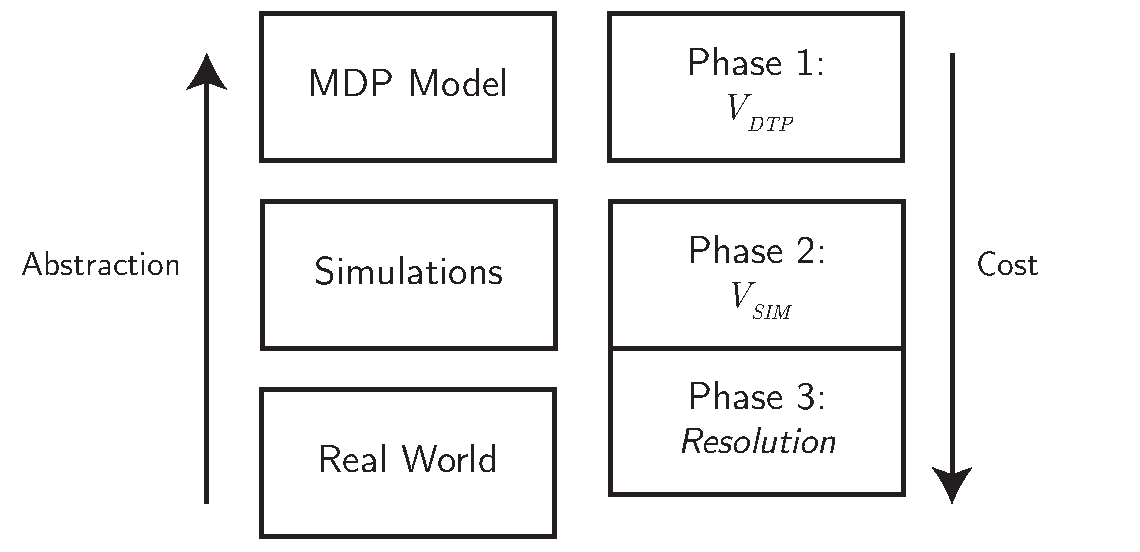
\includegraphics[width=0.7\textwidth]{abstraction-5-1}
	\caption{Correspondence of the phases of the model learning framework to the different levels of abstraction.}
	\label{fig:abstraction-cost}
\end{figure}

%\begin{itemize}
%	\item Change the $\beta$-parameter of Eq 5.1 over time
%	\item The $\gamma$ discount factor (low values $\to$ faster planning)
%	\item Three 'phases':
%\end{itemize}

\afterpage{
	\begin{figure}[t]
		\centering
		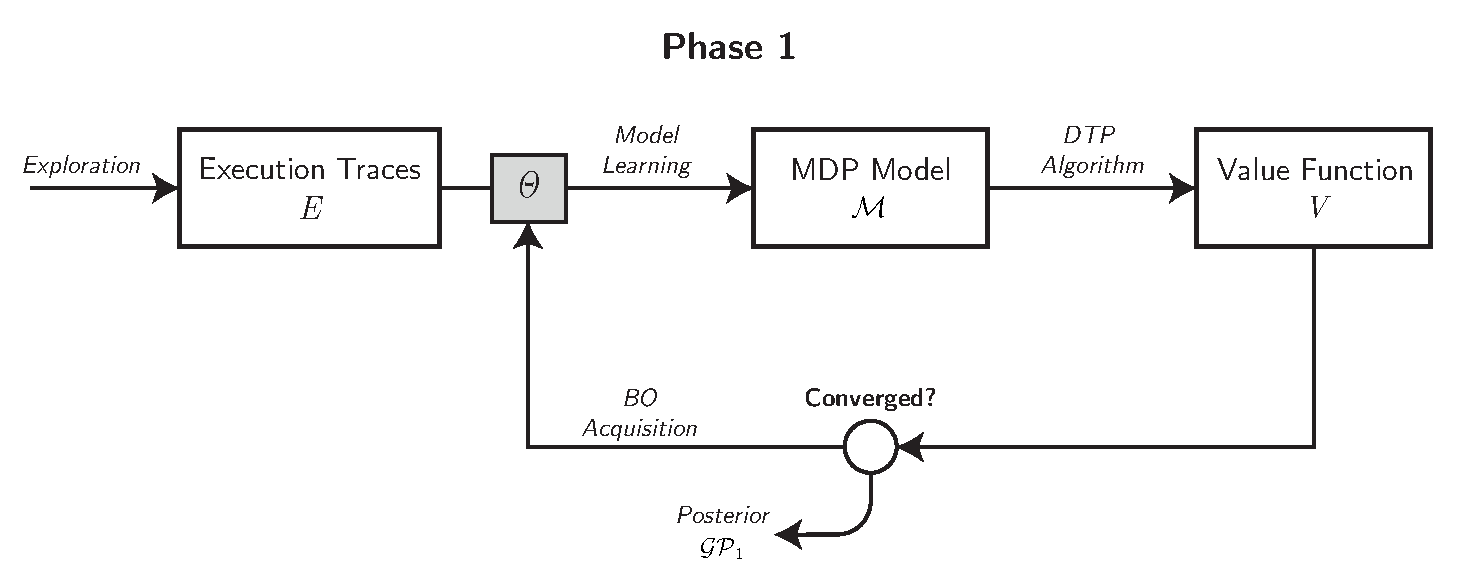
\includegraphics[width=1.0\textwidth]{phase-1v2.pdf}
		\caption{Block diagram showing the steps of the first phase of the multi-phase optimization framework. This phase develops a distribution which reflects the interesting area of the parameter space solely based on the value functions of \acrshortpl{acr:mdp}.}
		\label{fig:phase-1}
	\end{figure}
	
	\begin{figure}[t]
		\centering
		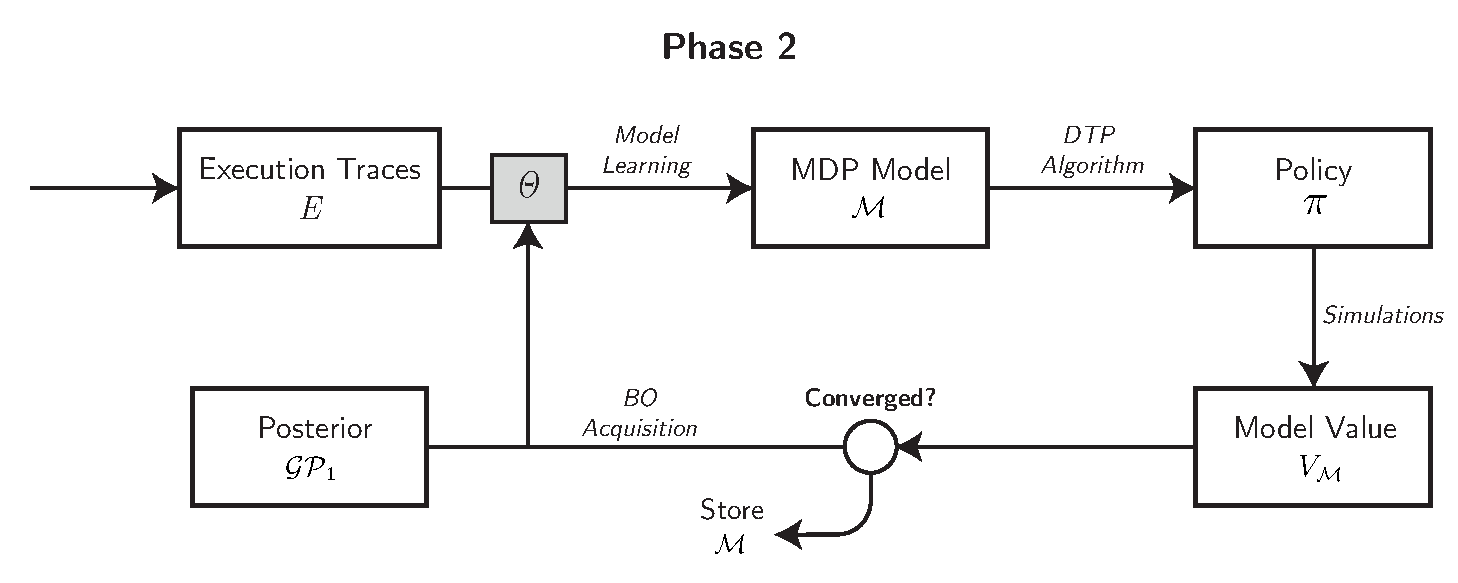
\includegraphics[width=1.0\textwidth]{phase-2v3.pdf}
		\caption{Block diagram showing the steps of the second phase of the multi-phase optimization framework. This phase uses the distribution learned in the first phase as a prior and optimizes for an \acrshort{acr:mdp} which maximizes performance in simulations.}
		\label{fig:phase-2}
	\end{figure}
	
	\begin{figure}[t!]
		\centering
		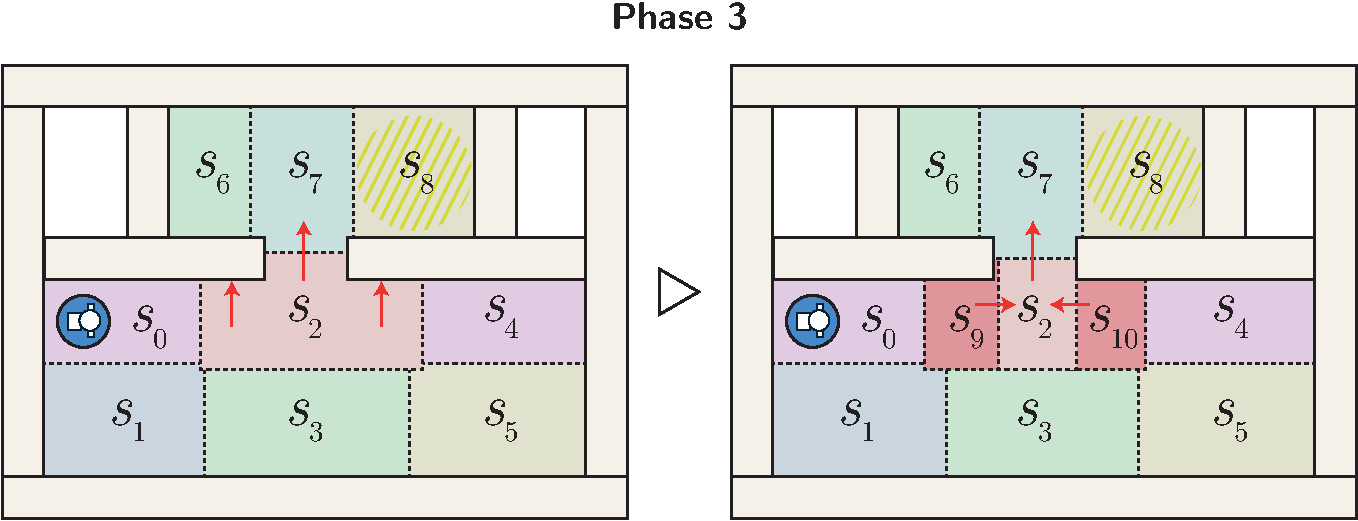
\includegraphics[width=1.0\textwidth]{phase-3.pdf}
		\caption{An illustration of the goal of the third phase in the context of mobile robot navigation. In the navigation towards the goal state $s_8$, the robot might get stuck in state $s_2$ following the optimal policy. Therefore, higher resolution is needed in this area of the state space.}
		\label{fig:phase-3}
	\end{figure}
	\clearpage
}

\subsection{Phase 1: Value Function Pre-Processing}
\label{sec:phase-1}

In the first phase the performance is assessed solely based on the value functions derived by the \acrshort{acr:dtp} algorithm used for planning.
This means the $\beta$ parameter is set to $\beta = 1.0$ such that the performance $V_{\mathcal{M}}$ of \acrshort{acr:mdp} $\mathcal{M}$ is expressed only in terms of $V_\mathit{DTP}$ and so no simulations are performed in this phase.
Therefore, this first phase is relatively cost-cheap, and although it abstracts from the real-world the most, it may be used to identify the interesting area of the parameter space.
Hence, the goal of this first phase is to narrow down the search space to a subspace of learning parameters more likely to yield high performance.

The block diagram in \autoref{fig:phase-1} depicts the main steps of this first phase, whose pseudo-code is presented in \autoref{alg:multi-phase-framework}, starting from \autoref{alg:line:phase1}.
In each iteration of this first phase the execution traces $E$ from the exploration are used to obtain an \acrshort{acr:mdp} by applying the learning algorithms given a parameter-setting $\theta$.
The value of the learned model $\mathcal{M}$ is then assessed based only on the value function $V$ for a set of tasks $T_\mathcal{M}$ the system is expected to perform.
The value of model $\mathcal{M}$ is thus computed as:
\begin{equation*} 
V_{\mathcal{M}} = \frac{\sum_{t \in T_\mathcal{M}} V_{\mathit{DTP}, t}}{|T_\mathcal{M}|}
\end{equation*}
where each task $t \in T_\mathcal{M}$ is defined in terms of an initial state and reward function.

Based on the gathered evidence new parameter-settings $\theta$ are sampled iteratively, which are those settings for which the utility is the highest in the acquisition function $a_1$ used for \acrshort{acr:bo}.
This continues until a stopping condition has been met, where in this first phase stopping after a fixed number of iterations should be acceptable, as the goal is only to narrow down the search space.
At the end of the first phase, the resulting posterior \acrshort{acr:gp} distribution $\mathit{gp}_1$ is taken and used for the acquisition in the next optimization phase.

%In practice this could be done by setting a threshold, say, $\eta \in [0, 1]$, that specifies the allowed deviation from the observed maximum in the evidence set $\mathcal{D}$, i.e. $\max_\mathcal{(x_i, y_i) \in D} y_i$, which can be used to define parameter bounds based on the posterior mean.

%\fbox{\textbf{TODO:} Update threshold to prior.}

%First phase: Performance assessment solely based on $V_\mathit{DTP}$ (i.e., initially $\beta = 1$). No simulations. $\gamma$ parameter starts off low and increases over time. This means this first phase is relatively cost-cheap, but might give us a global idea of the interesting area of the parameter-space so that we could narrow this space down.

%\blindtext

\newpage

\subsection{Phase 2: Simulation-Based Optimization}
\label{sec:phase-2}

\begin{figure}[t!]
	\centering
	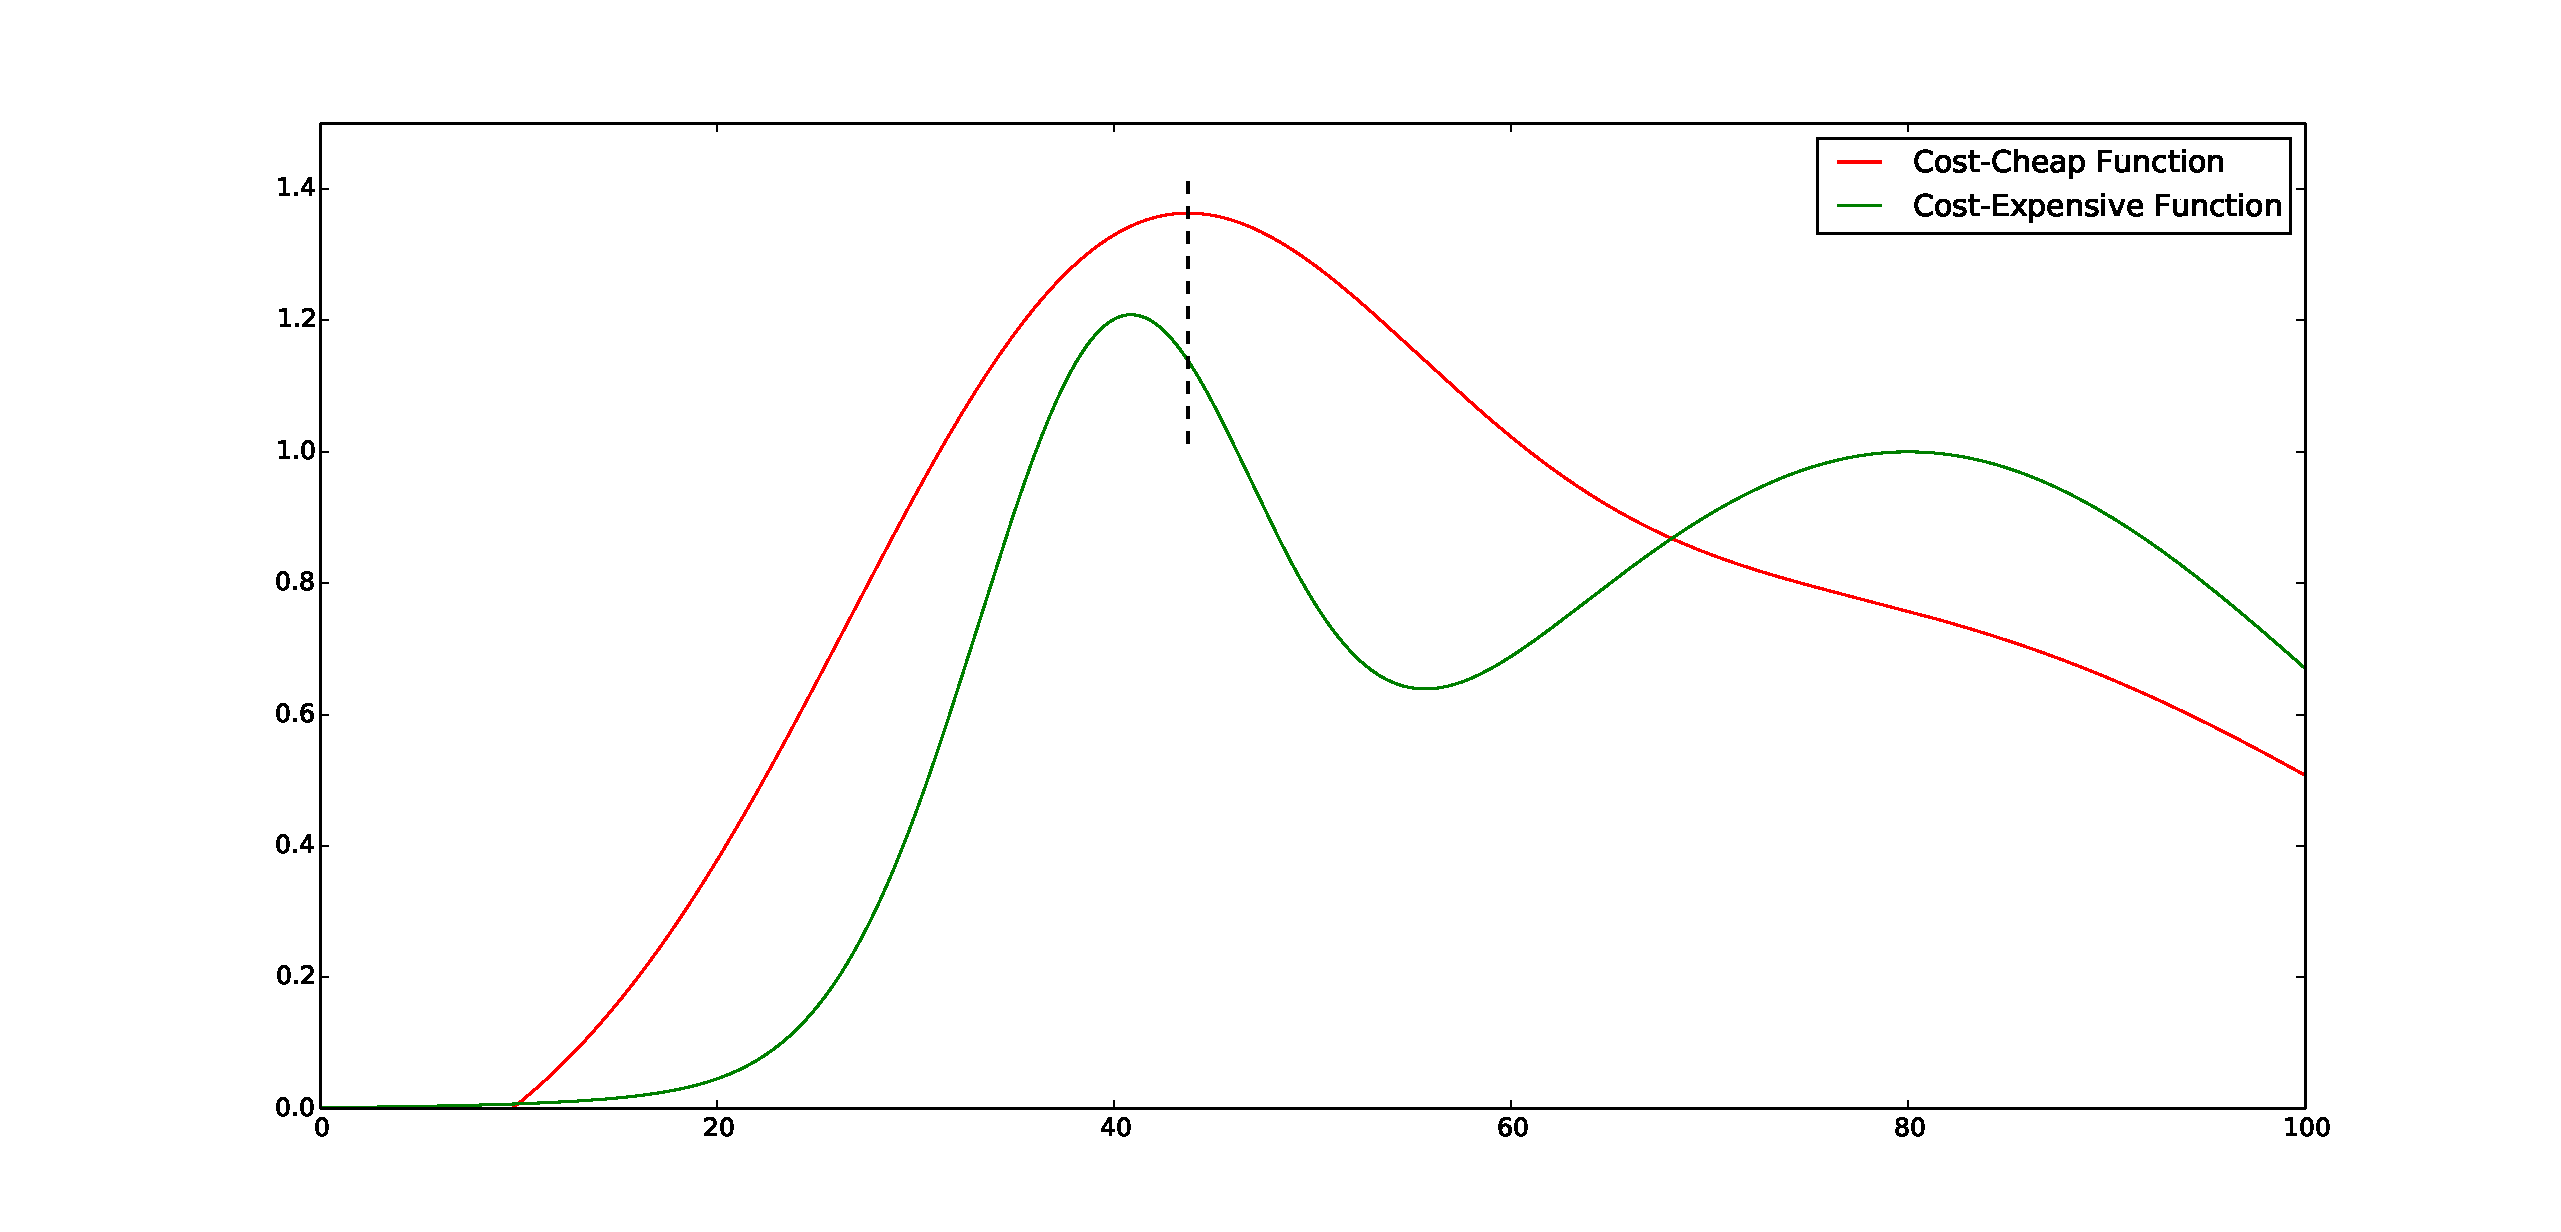
\includegraphics[width=0.75\textwidth]{phase-2-illustration-idea.pdf}
	\caption{An illustration of the idea behind the second phase of the multi-phase framework. }
	\label{fig:phase-2-idea}
\end{figure}%TODO New figure + remove white space (tight-layout?) + larger fonts

In the second phase the performance is assessed solely based on simulations of the system under consideration.
This means that, instead, the $\beta$ parameter is now fixed at $\beta = 0.0$ such that the performance $V_\mathcal{M}$ of \acrshort{acr:mdp} $\mathcal{M}$ is expressed only in terms of $V_\mathit{SIM}$.
Therefore, the second phase is much more cost-expensive and so a desirable aim is to minimize the number of evaluations needed.
In an attempt to do so, the second phase exploits the knowledge gathered in the first phase by utilizing the \acrshort{acr:gp} $\mathit{gp}_1$ in the acquisition of new samples in the optimization process.
The idea is thus to first sample from those parts of the parameter space $\Theta$ expected to yield high value according to the observations in the first phase.

The block diagram in \autoref{fig:phase-2} depicts the main steps of this second phase, whose pseudo-code is presented in \autoref{alg:multi-phase-framework}, starting from \autoref{alg:line:phase2}.
The first thing that differs from the previous phase is that, in each iteration, the value of the learned model $\mathcal{M}$ is assessed based on cost-expensive simulations.
The value of model $\mathcal{M}$ is thus computed as:
\begin{equation*}
V_\mathcal{M} = \frac{\sum_{t \in T_\mathcal{M}} V_{\mathit{SIM}, t}}{|T_\mathcal{M}|}
\end{equation*}
\noindent where each task $t \in T_\mathcal{M}$ is defined in terms of an initial state and reward function.

The main difference, however, lies in how new parameter-settings $\theta$ are sampled in each iteration in this phase.
The acquisition in this phase is based on the \textit{integrated acquisition function}, defined in \autoref{eq:integrated-acq}, as it uses the \acrshort{acr:gp} from the prior phase and the \acrshort{acr:gp} posterior based on the observations of this phase.
That is, the acquisition function is defined as:
$$\alpha\cdot\mathsf{EI}(x\vert\mathcal{D}_1, \mathit{gp}_1) + (1 - \alpha)\cdot\mathsf{EI}(x\vert\mathcal{D}_2, \mathit{gp}_2)$$
\noindent where $\mathcal{D}_1$ and $\mathcal{D}_2$ are the evidence sets, and $\mathit{gp}_1$ and $\mathit{gp}_2$ the \acrshortpl{acr:gp} approximations of the first and second phase respectively, with the expected improvement $\mathsf{EI}$ at $x \in \Theta$ weighed by $\alpha$.

The knowledge obtained in the first phase is utilized by weighing the expected improvement more heavily for selecting the first few samples (i.e., setting $\alpha$ to a high value).
Over time, the influence of the first phase decreases by lowering the value of $\alpha$ as more observations are made.
In this way, if the global maximum in the first phase lies close to that of the second phase, a performance-maximizing \acrshort{acr:mdp} may be found faster, as the sampling is initially steered by the approximation in the first phase.%TODO Refer to the example figure

%The second phase exploits the knowledge gathered in the first phase by using it as a \acrshort{acr:gp} prior in a new optimization process such that it starts off in the part of the parameter space most likely to yield high value.
%In this phase the performance assessment becomes more cost-expensive, but is also made more accurate by performing simulations and weighing the observed $V_\mathit{SIM}$ in the performance measure.
%This means, we either fix the $\beta$ parameter to a value in $[0, 1)$, or alternatively, gradually decrease it over time so that $V_\mathit{SIM}$ plays a more significant role the more iterations have passed.
%
%The block diagram of \autoref{fig:phase-2} depicts the main steps of this second phase.
%The same execution traces from the exploration are again passed to model learning algorithms to obtain \acrshortpl{acr:mdp} given parameter-settings $\theta$.
%What is first of all different is that the acquisition of new samples is steered by the prior obtained from the first phase.
%Secondly, the value is now determined by simulations in which the policies emerging from a learned model $\mathcal{M}$ are followed for the tasks that the agent is expected to perform.
%This value $V_\mathcal{M}$ is thus computed as in \autoref{eq:vm} with a weight factor $\beta > 0$.
%The optimization process continues until a stop condition, which could be either reaching a fixed number of iterations, a fixed time or a stopping criterion (e.g., when potential improvement becomes negligible).
%At this point we can obtain an \acrshort{acr:mdp} most likely to yield high performance for the problem under consideration.

%Second phase: $\beta$ decreases over time, which means $V_\mathit{SIM}$ starts to play a role, and assessment becomes more accurate, but also more cost-expensive.

%\blindtext

\subsection{Phase 3: Resolution Post-Processing}
\label{sec:phase-3}

\begin{algorithm}[t!]
	\caption{\acrshort{acr:mdp} Optimization Multi-Phase Framework (Phase 3)}
	\label{alg:multi-phase-fine-tuning}
	\begin{algorithmic}[1]
		\Require{\acrshort{acr:mdp} $\mathcal{M}_\mathsf{in} = (\mathcal{S}, s_0, A, \delta, R)$, Set of tasks $T$, Time-step $t$, Discount factor $\gamma \in [0, 1]$}
		\Ensure{\acrshort{acr:mdp} $\mathcal{M}_\mathsf{out}$}
		\Statex
		\Function{Phase3}{}
		\ForAll{$(\mathit{start}, \mathit{goal}) \in T$}
		\State $(s_0, s_g) \gets \textproc{ToStates}(\{\mathit{start}, \mathit{goal}\})$
		\State $R \gets \textproc{ToRewardFunction}(s_g)$
		\State $\mathcal{M} \gets (\mathcal{S}, s_0, A, \delta, R)$
		\State $V, \pi_t \gets \textproc{DTPPlanning}(\mathcal{M})$
		\State $\mathsf{task\_status}, \mathit{steps} \gets \textproc{RunSim}(\mathcal{M}, \pi_t)$
		\If{$\mathsf{task\_status} = \texttt{stuck}$}
		\State Let $s_f$ be the state in which the system got stuck
		\State $R \gets \textproc{ToRewardFunction}(s_f)$
		\State $\mathcal{M} \gets (\mathcal{S}, s_0, A, \delta, R)$
		\State $V, \pi_f \gets \textproc{DTPPlanning}(\mathcal{M})$
		\State Let $E_\mathit{SIM}$ be a dictionary
		\ForAll{$a \in A, s' \in \mathcal{S}$}
			\State $E_\mathit{SIM}[a][s'] \gets \emptyset$
		\EndFor
		\ForAll{$i \in \{1, \ldots, 100\}, a \in A$} \Comment{Perform trials of all actions from state $s_f$}
		\State Let $o$ be the current system state observations
		\State Execute $a$ and let $s'$ be the resulting state
		\State $E_\mathit{SIM}[a][s'] \gets E_\mathit{SIM}[a][s'] \cup \{o\}$	\Comment{Store the observed transition in $E_\mathit{SIM}$}
		\While{$s' \neq s_f$} \Comment{Move back to state $s_f$}
			\State Execute $\pi_f(s')$ and update $s'$ to the resulting state
		\EndWhile
		\EndFor
		\State $\mathit{new\_centroids} \gets \emptyset$
		\ForAll{$a \in A$}
			\If{$|E_\mathit{SIM}[a]| > 1$}
				\ForAll{$s' \in \mathcal{S}$}
					\State $\mathit{new\_centroids} \gets \mathit{new\_centroids} \cup \{\textproc{Average}(E_\mathit{SIM}[a][s'])\}$
				\EndFor
			\EndIf
		\EndFor
		\State Split the state $s_f$ into new states based on $\mathit{new\_centroids}$
		\State Update $\delta$ for the new states based on $E_\mathit{SIM}$
		\EndIf
		\EndFor
		\State\Return $\mathcal{M}$
		\EndFunction
	\end{algorithmic}
\end{algorithm}

The last phase starts when the parameter space has been narrowed down sufficiently or the parameter search has converged to an optimum.
In this phase, the goal is to further improve learned models by checking whether the transition probabilities are likely to match reality.
The identification of discrepancies in these probabilities happens by executing actions in those areas of the state-space that are visited most often and in which the agent tends to get stuck (according to the transition probabilities) and seeing if the observed transitions yield comparable probabilities.
For those areas and their corresponding states for which mismatches are identified, higher resolution is provided to better reflect the system's dynamics in the real world.

The illustration of \autoref{fig:phase-3} aims to clarify the goal of this third phase by means of an example for the context of mobile robot navigation.
Although the model obtained in the previous phase, might yield high performance for most of the tasks used to assess model value, a situation as illustrated in this figure might occur.
That is, in the figure the robot, depicted in blue, needs to move from its current position to the goal, indicated by the yellow shaded area.
For the state space depicted on the left-side however, the robot might get stuck following the optimal policy from which the need for higher resolution in this area emerges.
% To identify these discrepancies we could check if the transition probabilities of the model match observed outcomes of actions from the different states of the model.

%Third phase: Starts when the parameter-space has sufficiently been narrowed down. To further improve learned models we would like to see if the opportunity exists of having higher resolution in some areas of the state space to better reflect the data-set.

%\blindtext


%% OLD %%

%\textbf{Note:} These bullet-points have not been completely updated yet although most are still relevant. Outline should be such that we first discuss the framework for model learning and optimization without considering incomplete data or doing cost-sensitive optimization, which are discussed next ('why and how').
%Probably describing the framework should be separated from the application to mobile robot navigation and how it is implemented, which should be described afterwards.
%
%\begin{itemize}
%	\item Introduction
%	\item Explain high-level algorithm idea?
%\end{itemize}
%
%\section{Application}
%\label{sec:application}
%
%% 
%
%\begin{itemize}
%	\item Mobile robot navigation
%	\item Why this application?
%	\item Generalization possible to other applications?
%\end{itemize}
%
%\section{Exploration Phase}
%\label{sec:exploration-phase}
%
%% 
%
%\begin{itemize}
%	\item Obtain a dataset of observations, for our application this concerns data about attainable positions of the robot that will be controlled
%	\item Under the assumption such a dataset is not yet available to us, this dataset is retrieved in an exploration phase
%	\item In this exploration phase, the robot should explore the environment and periodically record information about its current position while aiming to visit all the locations of importance
%	\item This exploration phase is (preferably) only carried out once
%	\item To obtain a dataset for our tests the exploration phase is carried out in a robot simulator. Should also explain what data is obtained in this exploration.
%	\item The overall algorithm is tested for multiple maps/(office-like) environments, which might differ in their dimensions, number of obstacles or `openness'.
%	\item To take into account dynamically changing environments to some extent, there are also doors that will be open or closed as time passes.
%	\item The simulations are carried out in the Morse simulator, in which the exploration is carried out by an agent that randomly navigates an environment.
%\end{itemize}
%
%\section{State Space Acquisition}
%\label{sec:state-space-aggregation}
%
%% 
%
%\begin{itemize}
%	\item Using exploration data
%	\item Unsupervised machine learning to obtain states for an MDP model (various possible methods possible: e.g., kmeans, gmm)
%	\item Unknown parameter $\delta$ of the unsupervised machine learning algorithm to be optimized
%\end{itemize}
%
%\section{Model and Policy Acquisition}
%\label{sec:model-policy-acquisition}
%
%% 
%
%\begin{itemize}
%	\item State space obtained as described in previous section
%	\item Transition function obtained based on exploration data and state space through the likelihood maximization approach.
%	\item For our application the actions are fixed and can either be \textsc{NORTH}, \textsc{EAST}, \textsc{SOUTH}, \textsc{WEST} which makes the robot navigate in the corresponding direction.
%	\item Rewards
%	\item Timesteps
%	\item Policy (various possible `solvers': value iteration, policy iteration)
%\end{itemize}
%
%\section{Bayesian Model Optimization}
%\label{sec:bayesian-model-optimization}
%
%% 
%
%\begin{itemize}
%	\item Optimization of the unknown $\delta$ parameter of the machine learning algorithm for state space aggregation
%	\item Evaluation by simulations of the found policy for the given $\delta$ parameter
%	\item ...
%\end{itemize}
%
